\chapter{Treplica Reconfigurável}\label{cap2:treplica_reconfiguravel}

Cobiçamos para Treplica um mecanismo de autogestão capaz de realizar autointegração de
réplicas sem intervenção humana, inteligente o suficiente para detectar oscilação na
demanda e reagir a elas, proporcionando assim maior eficiência na utilização de recursos
físicos. Projetar mecanismos autônomos sintonizados para reagir rapidamente às mudanças no
sistema é um assunto atual e relevante para pesquisa.

O primeiro passo para suportar tal anseio é dado nesse trabalho, que tem como objetivo
transformar Treplica em uma biblioteca reconfigurável. O problema de reconfiguração é
complexo, principalmente na presença de falhas e assincronia. Sua resolução é obtida
basicamente a partir de duas maneiras: (1) abordagem baseada em transições de visões do
conjunto de réplicas participantes (e corretas) \cite{birman87a, birman87b}; (2)
definição, via consenso, de uma nova configuração a partir da construção de uma barreira
que, quando alcançada pelas réplicas, faz com que elas abandonem a configuração vigente e
ingressem na nova configuração definida (caso elas façam parte dela) \cite{lamport10}.

O processo de reconfiguração pode ser bem complexo, como descrito em \cite{lamport10},
então nessa dissertação estaremos interessados em um sub-conjunto desse problema onde
apenas novas réplicas são adicionadas. Isso é mais simples porque o estado inicial de uma
nova réplica é sempre vazio, consequentemente não precisamos de uma política para tratar
réplicas com estado. Em outras palavras, a política para tratar recuperação de falhas em
Treplica não foi alterada.

Para implementar esse mecanismo, identificamos a necessidade de um mecanismo eficiente
capaz de transferir estado entre réplicas. Treplica ainda não possui tal mecanismo capaz
de adicionar novas réplicas e recuperação de falhas. Estamos preocupados com o impacto
inerente para implantar uma nova réplica em um aglomerado em tempo de execução. Tal
impacto dificulta a viabilidade das técnicas de autogestão, porque dependendo do cenário,
adicionar uma nova réplica pode comprometer o desempenho de um sistema sobrecarregado
\cite{vilaca09}.

Neste capítulo apresentaremos as alterações propostas em Treplica, começando pelos
principais componentes da biblioteca que serão de fundamental importância para compreensão
das alterações propostas na biblioteca. Iniciaremos com a \autoref{sec:visao_arquitetural}
apresentando os componentes de suporte fundamentais para arquitetura de Trepica e
examinamos detalhadamente os componentes utilizados para construção do algoritmo Paxos. Em
seguida, na \autoref{sec:alteracoes_propostas} apresentamos minunciosamente as alterações
e os novos componentes propostos para Treplica.


\section{Visão arquitetural de Treplica}\label{sec:visao_arquitetural}

A arquitetura de Treplica é baseada em uma \emph{fila persistente assíncrona}
\autoref{fig:paxos_persistent_queue}, sua implementação segue muito de perto a
decomposição modular de Paxos apresentada por \citeonline{lamport06a}. A fila é composta
por classes internas da biblioteca que representam a funcionalidade dos quatro agentes
de Paxos:

\begin{figure}[ht]
  \centering
  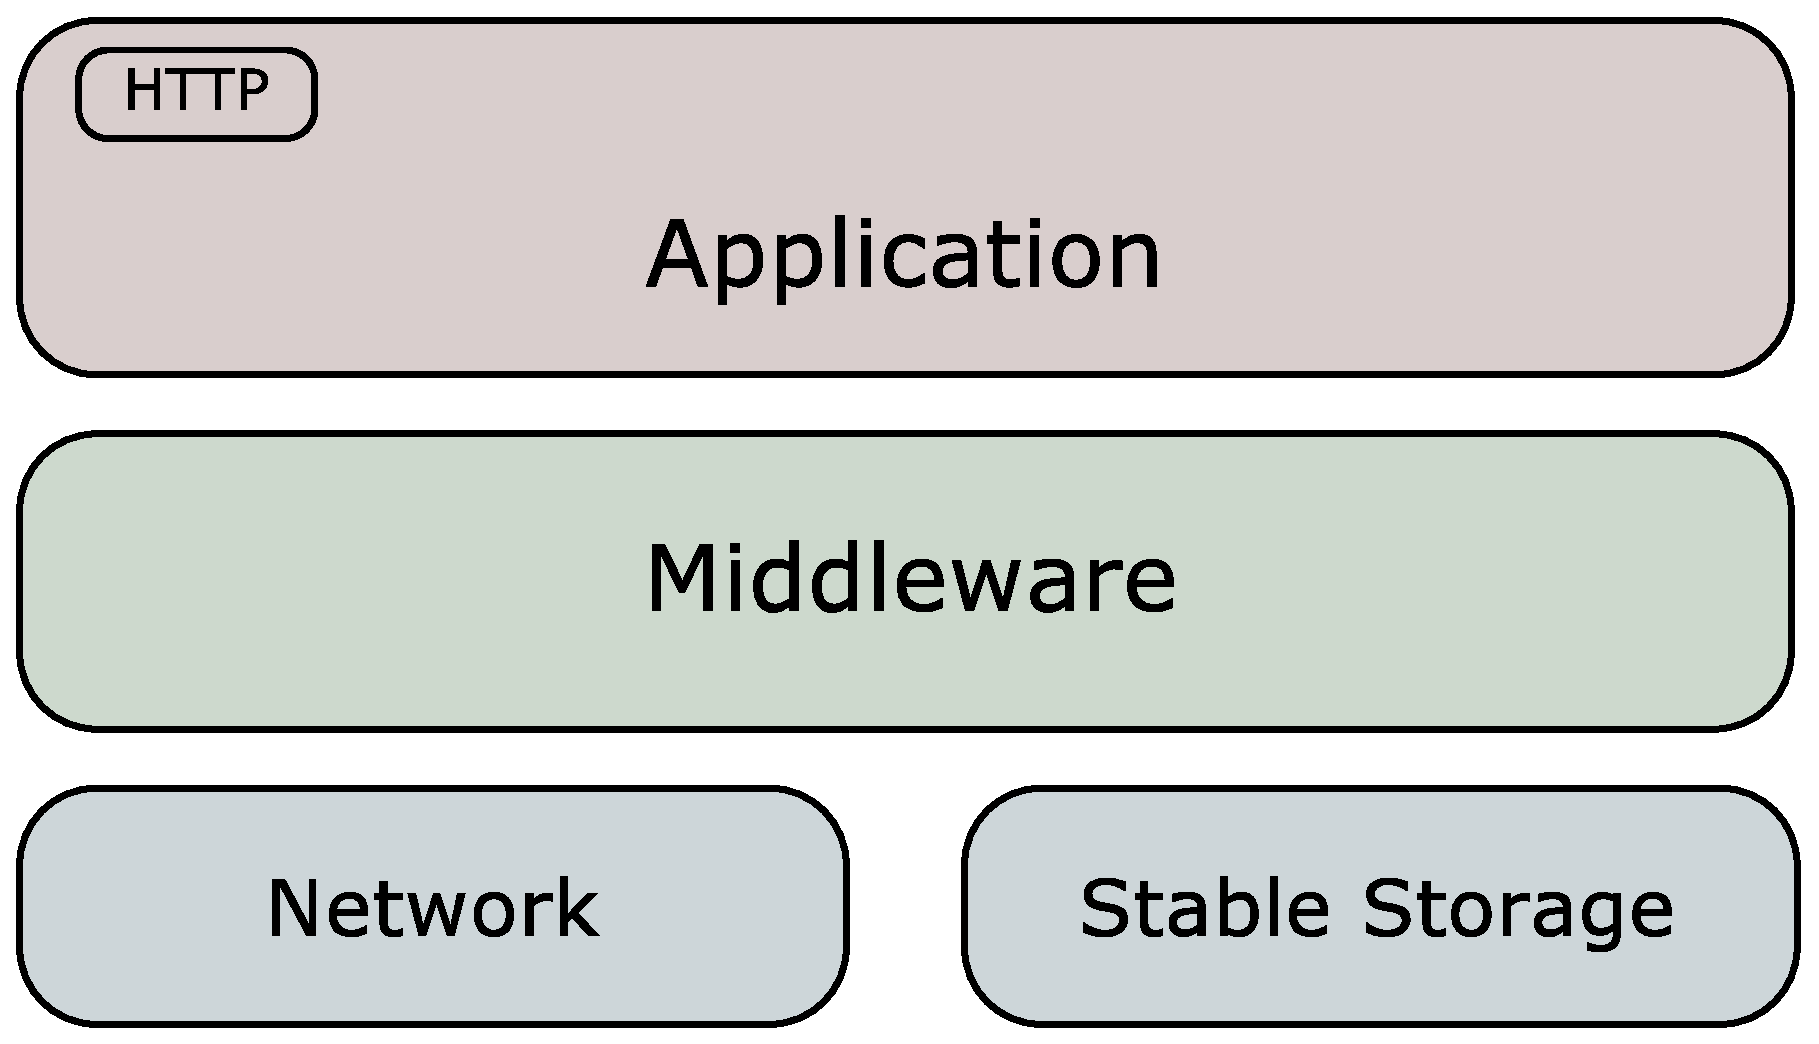
\includegraphics[width=12cm]{conteudo/capitulos/figuras/block-simple.eps}
  \caption{Paxos Persistent Queue}
  \label{fig:paxos_persistent_queue}
\end{figure}

\begin{itemize}
  \item \classname{Learner}: combina os agentes proponentes e aprendiz em uma única classe
    responsável pelo monitoramento do fluxo de instâncias de Paxos, convertendo
    mensagens em objetos para serem entregues para fila;
  \item \classname{Acceptor}: atua como um receptor;
  \item \classname{Coordinator}: atua como um coordenador;
  \item \classname{Election}: algoritmo para eleição do líder, usado para selecionar um
    único coordenador.
\end{itemize}

As classes que implementam esses agentes foram concebidas para serem independentes,
tornando possível a criação de réplicas que executam Paxos com diferentes subconjunto de
agentes. Especificamente, uma réplica contendo apenas o agente \classname{Learner} poderá
propor e aprender valores, efetivamente executando uma fila completa, sem participar do
processo de consenso (votação). Uma réplica configurado dessa forma poderia ser usada para
aumentar a capacidade de expansão do sistema.

As principais classes de suporte possuem estruturas semelhantes ao dos agentes de Paxos:
são módulos encapsuladores de comportamento estritamente reativos. Eles operam através
da transformação de mensagens endereçadas a eles pela classe \classname{Router} e também
podem enviar novas mensagens à rede, armazenar informação na memória não-volátil ou
entregar objetos para aplicação. Essas tarefas são manipulados pela classe
\classname{Secretary}, que oferece uma interface uniforme a todas as tarefas de E/S
requeridas pelos agentes. A abstração fornecida pelo \classname{Secretary} oferece aos
agentes uma forma de enviar mensagens e acessar a memória estável. Essa classe baseia seus
serviços nas classes \classname{Transport} e \classname{ChangeLog} para acessar,
respectivamente, a rede e o armazenamento estável. Por sua vez, essas duas classes
fornecem abstrações que protegem os demais módulos dos detalhes de implementação. O
componente de transporte é implementado com base em \emph{multicast} sobre redes UDP/IP e
o \classname{ChangeLog} é baseado em sistema de arquivos simples.

Nas seções a seguir descreveremos esses módulos com mais detalhes. Eles são apresentados
de baixo para cima, começando com os módulos de suporte e, em seguida, descrevendo os
agentes de Paxos. Para cada módulo vamos mostrar a sua principal função, como ele interage
com outros módulos e as implicações de sua estrutura para a execução Paxos. O principal
foco é apresentar os componentes alterados na biblioteca que propusemos nessa dissertação.
A descrição completa desses componentes encontra-se em \citeonline{vieira-tr10b}.

\subsection{Módulos de suporte}

Em Treplica, os módulos de suporte são uma abstração dos mecanismos subjacentes a Paxos,
claramente definidos por interfaces que oferecem a flexibilidade necessária para
substituir o comportamento de um componente. A principal motivação para essa segregação
foi simplificar a API utilizada pelos agentes de Paxos. Dessa forma esses componentes
encapsulam os detalhes inerentes sobre endereçamento de réplicas, envio de mensagens
\emph{multicast} e \emph{unicast}, gerenciamento de memória não volátil (disco) e detecção
de falhas.

\subsubsection{Transport}\label{subsec:transport}

A abstração do transporte de dados é definida pela interface \classname{Transport}. Ela
oferece a seus clientes um mecanismo de envio e recebimento de mensagens \emph{multicast}
e \emph{unicast}. Suas propriedades estão alinhadas com as premissas da rede para uma
aplicação construída no modelo computacional assíncrono, ou seja, são enlaces de
perda-justa (\cite{sec:modelo_computacional}):

Canais perda-justa podem perder, duplicar ou trocar a ordem de mensagens. Mesmo assim,
essa abstração é adequada para o \classname{Transport} por duas razões: (1)
correspondência com as exigências da rede imposta por muitos algoritmos de consenso no
modelo assíncrono, incluindo Paxos; e (2) reflete de perto as garantias efetivamente
prestadas pelo modelo de transporte de rede utilizado pelo componente: UDP/IP.

Paxos não exige um modelo de transporte com propriedades de entrega de mensagens
confiável, pois essa propriedade está intrinsecamente implementada pelo próprio algoritmo,
incluindo mecanismos de buferização de mensagens e retransmissão). Se utilizarmos um
mecanismo de transporte confiável, duplicaremos as propriedades para garantia de
confiabilidade. Além disso, a entrega confiável fornecida por um transporte como TCP/IP só
funciona para o modelo de falhas falha-e-para\footnote{No modelo falha-e-para, um processo
não tem capacidade de se recuperar de uma falha, ou seja, a partir do momento que o
processo falha ele permanecerá falho até o infinito\cite{cachin11}} \cite{abdellatif04}.
No modelo falha-e-recuperação, o algoritmo de consenso ainda precisa verificar se as
mensagens foram entregues mesmo quando se usa TCP/IP.

\subsubsection{ChangeLog}

A abstração criada na classe \classname{ChangeLog} protege os agentes de Paxos dos
detalhes pertinentes ao armazenamento não-volátil (disco). Basicamente, o serviço
fornecido é um \emph{log} persistente de todas as mudanças ocorridas em um objeto, com
suporte para \emph{checkpointing}. Na verdade, a interface desse componente é muito
simples oferecendo métodos para escrita de alterações (acréscimo no \emph{log}), com o
apoio explícito para a recuperação. As alterações nos objetos podem ser acrescentadas ao
final do arquivo de \emph{log} de forma persistente e um objeto pode ser mais tarde
reconstruído a partir da repetição dessas mudanças armazenadas. Com relação ao mecanismo
de \emph{checkpointing}, vale ressaltar que ele é utilizado para melhorar o desempenho da
reconstrução de objetos a partir do \emph{log}. Ele armazena, de forma intercalada, cópias
completas do objetos, possibilitando a reconstrução de objetos em um único passo,
dispensando a necessidade da aplicação de todas as alterações para chegar no último estado
do objeto.

\subsubsection{Ledger}

A classe \classname{Ledger} é a abstração do estado persistente para implementação de
Paxos. É uma estrutura de dados comum, compartilhada por todos os agentes de Paxos,
implementados por Treplica, que conseguem através de uma interface acessar os dados de uma
instância de consenso bem sucedido. A implementação dessa interface suporta persistência
dos dados de forma não-volátil.

A classe \classname{LoggingLedger} é utilizada para persistir em \emph{log} (disco) as
alterações, quando utilizada em conjunto com \classname{ChangeLog}. Para simplificar o uso
de \emph{log} de alterações, esta implementação tem suporte para detectar e isolar as
alterações feitas em seu estado interno. A gravação de mudanças de estado e o acesso aos
dados persistidos são funcionalidades da classe \classname{ChangeLog}, enquanto
\classname{LogginLeger} registra e replica as mudanças. O \classname{Ledger} armazena o
estado completo de cada instância do consenso por réplica, mantendo todos os dados
exigidos por todos os tipos de agentes de Paxos implementados por Treplica
(\autoref{subsec:estado_persistente}). Dessa forma, é possível que qualquer agente
recupere seu estado, inclusive o coordenador.

\subsubsection{Secretary}

A classe \classname{Secretary} apresenta uma abstração unificada de E/S para os agentes de
Paxos. Esse componente utiliza memória persistente usando os componentes
\classname{ChangeLog} e \classname{Ledger}, lida com a passagem de mensagens usando o
módulo de \classname{Transport} e lida também com a fila de objetos utilizada para entregar
objetos para a aplicação. A principal razão para criação dessa abstração em Treplica foi
sintetizar as operações de E/S em \emph{threads} diferentes das que executam as operações
de Paxos. Operações de E/S em disco, tem grande potencial para reduzir o desempenho do
algoritmo Paxos por duas razões: (1) todas as requisições de escrita que estabeleceram
consenso, devem ser persistidas de forma não-volátil antes do progresso do algoritmo; (2)
alguns passos do algoritmo de Paxos podem demandar vários acessos à memória persistente.

\citeonline{vieira-tr10b} mostram que o E/S é tratado apenas pelo \classname{Secretary} de
forma assíncrona, possibilitando a ocorrência de paralelismo entre rodadas diferentes,
mesmo com apenas acessos sequenciais ao disco. Isso é feito através de uma fila que agrupa
gravações lógicas distintas e retém os dados para realizar uma única gravação física
quando disco estiver livre. Essa abordagem é vantajosa porque o tamanho dos dados de
escrita no disco afeta muito pouco a latência da chamada de sistema \emph{sync()} usada
para tornar a escrita estável. Dessa forma implementação de \classname{Secretary} absorve
a latência da \emph{system call} mantendo uma \emph{thread} separada para persistência dos
dados.

\subsubsection{PersistentQueue}

O componente de fila persistente assíncrona depende das abstrações fornecidas pelo
\classname{Secretary}. O serviço prestado por essas abstrações de baixo nível não são
definidas na especificação de Paxos. Assim, Treplica não supõe uma única implementação
para o componente de fila persistente.

Filas persistentes assíncronas são uma maneira para que um grupo de réplicas compartilhem
informações na forma de objetos. Esses objetos são enviados por qualquer réplica ligado à
fila e são transmitidos para as outras réplicas de forma totalmente ordenada e com entrega
garantida, independentemente de falhas. Esse comportamento pode ser mais precisamente
descrito pelas seguintes propriedades:

\begin{itemize}
  \item Objetos são entregues na mesma ordem para todas as réplicas.
  \item Objetos são entregues para todas as réplicas, mesmo que uma réplica falhe e mais
    tarde se recupere.
  \item Objetos são persistentes e sobrevivem a falhas em todas as réplicas.
\end{itemize}

Em Treplica, esse componente é definido como uma interface genérica que pode ser
implementada utilizando outras abordagens diferentes de consenso, desde que respeite as
propriedades definidas acima. Apesar da viabilidade para suportar diversas implementações,
Treplica utiliza somente uma implementação baseada em consenso para o componente de fila
persistente, definida pela classe \classname{PaxosPersistentQueue}.

\subsubsection{Router}

A classe \classname{Router} é um componente simples, mas vital para classe
\classname{PaxosPersistentQueue}, porque inicia todo o conjunto de agentes necessário para
o funcionamento de Paxos. Sua função principal é prover o \emph{main loop} da
implementação de Paxos, que recebe mensagens do componente de transporte e, de acordo com
o tipo da mensagem, encaminha para processamento no agente apropriado. Dessa forma, a
execução desse agente é sequencial e não precisa de controle de concorrência.

Esse é o único componente (\emph{thread}) que monitora o temporizador central e gera
eventos de \emph{timer}\footnote{Os eventos de \emph{timer} simbolizam a passagem do
tempo para a aplicação. Esse evento atinge todos os componentes que necessitam de um
relógio para seu correto funcionamento}. O código de processamento dos agentes não possui
operações demoradas ou bloqueantes, eles são programados como simples manipuladores de
eventos caracterizando uma arquitetura de processamento assíncrono baseada em eventos
(\emph{event-driven}). É responsabilidade do \classname{Router} instanciar agentes e
componentes de apoio e, também, inicializar a \classname{PaxosPersistentQueue}.

\subsection{Agentes de Paxos}\label{subsec:agentes_paxos}

Em Treplica, os agentes de Paxos efetivamente implementam o algoritmo Paxos.
Esses agentes são baseados na especificação do algoritmo e são responsáveis pelo seu
correto funcionamento. Os agentes descritos aqui utilizam os componentes de suporte
descritos na seção anterior.

\subsubsection{Election}

Esse agente é responsável pela eleição do líder requerido pelo protocolo Paxos para
garantir progresso no algoritmo. Ele expõe a seus clientes a interface de um detector de
falhas $\Omega$. Resumidamente, esse detector de falhas garante que todo agente de eleição
confie em uma réplica do sistema como correta e que existe um tempo futuro em que todos os
agentes de eleição confiarão na mesma réplica \cite{chandra96}. Se a réplica que todos os
agentes acreditam estar correta executar o agente coordenador, a propriedade de progresso
é garantida.

Por definição, Paxos deve ter um único agente coordenador em execução. O agente de eleição
não exige que os clientes consultem seu serviço para perceber mudanças de liderança.
Especificamente, ele é capaz de detectar quando a réplica é eleita como líder e inicia a
execução do agente coordenador em resposta a esse evento. Por outro lado, quando ele
detecta que a réplica deixou a liderança o agente coordenador é parado.

\subsubsection{Learner e Proposer}

Em Treplica, a classe \classname{Learner} implementa as funcionalidades de aprendiz e
proponente de Paxos. Ele é responsável por: (1) tratamento das requisições oriundas dos
clientes da fila persistente; (2) criação de propostas que encapsulam essas requisições; e
(3) acompanhamento das propostas até que elas sejam ordenadas e entregues.

Para entender por que há uma combinação entre a funcionalidade desses dois agentes no
mesmo módulo, basta observar as atividades realizadas por esse agente. É possível
classificar as duas primeiras tarefas como pertencentes ao agente proponente e só a última
tarefa como atividades do aprendiz. No entanto, a terceira tarefa é fundamental para
o funcionamento correto da implementação de Treplica utilizando a fila persistente e exige
conhecimento detido por ambos proponente e aprendiz. Isso acontece porque Treplica
suporta Paxos e \emph{Fast Paxos} \cite{lamport06a} na mesma implementação e \emph{Fast
Paxos} retira do agente coordenador a responsabilidade exclusiva de propor valores para
consenso.

A diferença de implementação entre Paxos e Fast Paxos não fazem parte do escopo desse
trabalho. Para maiores detalhes consulte \citeonline{vieira09}.

Devido a independência dos componentes em Treplica (descentralização), na Fase 1a os
agentes proponentes diferentes podem propor diferentes propostas para uma mesma instância
de consenso, provocando uma colisão. Essas colisões impossibilitam a determinação de
consenso e exigem medidas da biblioteca para solucionar o impasse. Quando essa situação é
detectada, o agente aprendiz troca de instância até conseguir exclusividade de instância
necessária para iniciar uma rodada de votação.

\subsubsection{Coordinator}

Coordenador é o agente responsável por conduzir a rodada de consenso, como descrito na
\autoref{subsec:algoritmo_basico}. Ele é o agente que envia a mensagem iniciando uma nova
rodada $r$ na Fase 1a. Após a formação de um quórum em $r$, o coordenador atua novamente,
na Fase 2a, ordenando a votação de uma determinada proposta. Na Fase 2b, o coordenador
computa os votos e estabelece o consenso de $r$.

É permitido a existência de apenas um coordenador por rodada, em caso de falha na réplica
que executa o agente coordenador, uma eleição de líder deve ser convocada para estabelecer
que uma réplica correta execute o agente coordenador. Como o algoritmo é executado no
modelo computacional falha-e-recuperação, uma réplica coordenadora defeituosa pode voltar
à computação acreditando que ainda é coordenadora. Nesse caso, uma nova eleição de líder
deve ser convocada para restabelecer a unicidade de coordenador por rodada.

\subsubsection{Acceptor}

O receptor é um agente responsável pela votação das propostas de consenso do algoritmo
Paxos. Esse agente reflete muito de perto o comportamento de Paxos descrito no
\autoref{cap1:replicacao_ativa_paxos}. O agente receptor aguarda pela mensagem da Fase 1a
que inicia uma nova rodada de consenso e responde, se for o caso, com o valor que ele
votou em alguma rodada anterior. Isso permite que a rodada progrida e habilita o
receptor a votar na rodada corrente, assim que receber a mensagem adequada na Fase 2a. Em
Treplica esse comportamento tem apenas duas pequenas modificações que aumentam o
desempenho do sistema \cite{vieira-tr10b}: (1) o receptor reduz o voto para uma pequena
mensagem de tamanho constante e (2) ele avisa ativamente o coordenador sobre instâncias
consensos decididas.

\subsubsection{PaxosPersistentQueue}

\classname{PaxosPersistentQueue} é responsável por agrupar todos os agentes de Paxos.
Essa classe possui o \emph{main loop} responsável pelo recebimento das mensagens trocadas
pela biblioteca, sejam elas mensagens de Paxos ou mensagens de configuração. A classe
\classname{PaxosPersistentQueue} foi criada para fornecer uma implementação para fila
persistente, base da arquitetura de Treplica, utilizada como canal ordenado para troca de
informações.


\section{Alterações propostas}\label{sec:alteracoes_propostas}

Apresentamos os conceitos utilizados para criação da biblioteca Treplica, os detalhes de
seus componentes e como eles estão relacionados. A partir de agora, iremos focar nossa
discussão nas alterações propostas para expansão da biblioteca. O objetivo dessa seção é a
apresentar e detalhar as seguintes funcionalidades:

\begin{itemize}
  \item Protocolo para transferência de estado: mecanismo eficiente para transferência de
    estado entre réplicas.
  \item Réplicas leitoras: a ideia principal dessa abordagem é reconfigurar o sistema de
    forma mais simples, utilizando réplicas réplicas que não participam de processo de
    decisão de instâncias de consenso.
  \item Equalização de estado: proposta para novo componente que preenche de forma
    eficiente lacunas na sequência de instâncias de consenso, caso uma réplica fique
    atrasada em relação às demais.
\end{itemize}

\subsection{Protocolo para transferência de estado}

A ideia principal dessa abordagem é a criação de um mecanismo que possibilite transferir, de
forma eficiente, o estado entre réplicas. Para isso, criamos um protocolo que orquestra as
interações entre réplicas e os bloqueios de estado necessários para garantia de
consistência. Visando maior clareza de exposição, quando necessário, chamaremos as
réplicas que recebem o estado como \emph{réplicas receptoras} e réplicas que transferem
seu estado como \emph{réplicas doadoras}.

A necessidade de um mecanismo para transferência de estado surgiu a partir da suposição da
equalização de estados divergentes entre réplicas da mesma aplicação. A disparidade de
estados em uma ambiente que emprega replicação ativa utilizando Paxos pode suceder a
partir de: (1) falha-e-recuperação de uma réplica ou falha transiente do enlace de
comunicação. Durante o período defeituoso, uma réplica pode perder $n$ decisões de
consenso criando uma grande lacuna entre seu estado local e o estado corrente da
aplicação; ou (2) a divergência de estados pode ter um motivo mais nobre: expansão do
aglomerado. No entanto, segundo \citeonline{lamport10}, toda operação para adição de
réplica em Paxos deve ser precedida de uma operação não trivial de reconfiguração.

Independente da motivação para aplicação de uma transferência de estado, essa operação
não deve gerar grande impacto para o processamento de requisições e deve preservar a
correção do algoritmo. Tendo em vista a garantia de consistência, implementamos essa
operação como uma tarefa \emph{síncrona}\footnote{No modelo requisição/resposta, o emissor
dos dados fica bloqueado até receber uma resposta do receptor \cite{coulouris11}}. As
seguintes premissas foram supostas para construção do protocolo:

\begin{itemize}
  \item Quando uma réplica inicia o processo de transferência, todas as mensagens
    recebidas não pertencentes ao protocolo de transferência devem ser ignoradas.
  \item A réplica doadora não deve processar nenhuma operação de escrita enquanto realiza
    a transferência de estado.
  \item Novas réplicas estarão aptas para processar requisições (leitura ou escrita)
    somente após a configuração de um estado inicial.
\end{itemize}

Baseado nessas premissas, podemos afirmar que a operação de transferência de estado é
custosa para o desempenho de Paxos, pois estamos bloqueando temporariamente a participação
de uma réplica no processo de decisão de instâncias de consenso.

\subsubsection{Funcionamento do protocolo}\label{subsec:funcionamento_protocolo}

Estabelecemos a premissa que é responsabilidade da réplica receptora encontrar uma réplica
doadora (réplica disposta a transferir o seu estado). A simplicidade do mecanismo de
seleção de doador é herdada de Treplica: as réplicas conhecem somente seu próprio
identificador de rede e podem alcançar todas as outras réplicas por uma primitiva simples
de difusão. Criamos o protocolo com a preocupação de minimizar a degradação de desempenho
causada pela operação de transferência de estado. Ele foi dividido em três fases, conforme
ilustra a \autoref{fig:fases_protocolo}.

\begin{itemize}
  \item Na Fase 1 (\emph{Fase de Negociação}) a réplica receptora faz a solicitação de
    transferência de estado, obedecendo a uma \emph{política contratual}.
  \item Na Fase 2 (\emph{Seleção de Doadora}) ocorre a apuração do melhor acordo proposto
    pelas réplicas que atendem às exigências estabelecidas pela réplica receptora. Somente
    uma réplica doadora é selecionada.
  \item Finalmente, na Fase 3 (\emph{Transferência}) o estado da réplica doadora eleita na
    Fase 2 é transferido para a réplica receptora.
\end{itemize}

\begin{figure}[ht]
  \centering
  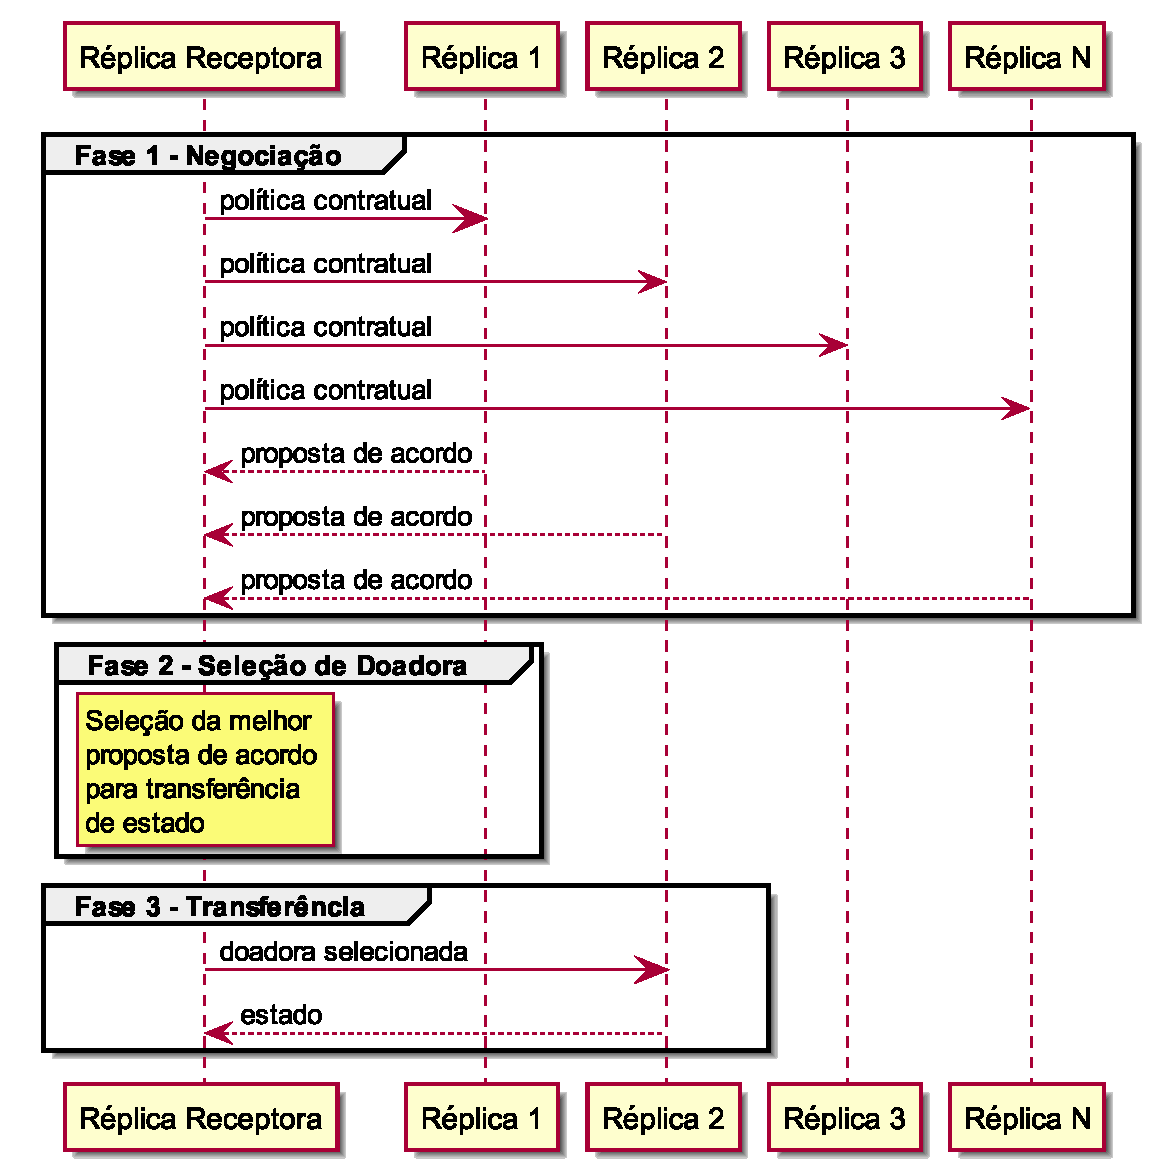
\includegraphics[width=11cm]{conteudo/capitulos/figuras/fases_protocolo_transferencia.eps}
  \caption{Fases do protocolo de transferência de estado}
  \label{fig:fases_protocolo}
\end{figure}

Na Fase de Negociação a réplica receptora estabelece as regras da transferência de estado
através da mensagem \classname{PolicyMessage}. Por exemplo, supomos que, independente do
motivo, uma réplica $r$ deseje receber um estado a partir da instância de consenso $i$.
Então, $r$ inicia a negociação de estado difundindo uma mensagem com essa política
contratual, o predicado: a maior instância de consenso decidida é maior que $i$. As
réplicas que recebem essa mensagem de solicitação de negociação de estado são solidárias e
tentam atender essa requisição. Elas avaliam as exigências contidas na mensagem e, caso
estejam de acordo, enviam somente para a replica receptora (remetente do contrato) a
mensagem \classname{DealMessage}. Essa proposta de acordo, contém informações referentes
ao estado que a réplica doadora está oferecendo. Caso a réplica receptora não receba
nenhuma proposta de acordo após um tempo pré-estabelecido, ela reinicia a Fase de
Negociação até encontrar uma réplica doadora. Podemos nos beneficiar dessa etapa inicial
do protocolo para criarmos diferentes políticas contratuais para transferência de estado.
Nessa versão proposta de Treplica, supomos configurações de duas politicas: uma mais
agressiva e outra mais ingênua. Lembrando que todas as políticas devem incluir qual é a
instância de consenso pretendida.

\begin{itemize}
  \item Somente réplicas leitoras: essa política é mais restritiva, busca um acordo com
    uma réplica leitora\footnote{Réplicas leitoras são aquelas onde apenas os agentes
    proponente e aprendiz estão em execução. Elas não assumem um papel fundamental na
    execução de Paxos. Descreveremos réplicas leitoras na
    \autoref{sec:replicas_leitoras}}.
    Acordos com réplica leitoras são preferíveis devido à restrição de sincronia exigida
    pelo protocolo. Dessa forma, essa política tenta minimizar possíveis impactos na
    computação de Paxos.
  \item Qualquer réplica: essa política é a menos restritiva possível, busca um acordo
    independente da configuração da réplica.
\end{itemize}

Devemos ter cuidado ao eleger qualquer réplica como réplica doadora, pois podemos gerar
impacto direto no desempenho da aplicação. A réplica doadora não participará da decisão de
um nova requisição durante o período que está transmitindo seu estado para garantir a
consistência. Lembrando que, no algoritmo Paxos, a partir do momento em que a maioria dos
receptores concordam com a alteração do estado, mais cedo ou mais tarde todas as réplicas
chegarão ao mesmo estado. A partir do momento que retiramos temporariamente da computação
uma réplica votante, a probabilidade de atingir consenso pela maioria diminui, podendo até
impossibilitar o progresso do algoritmo.

O protocolo progride quando a réplica receptora possui propostas de acordo. Quando essa
condição é alcançada, ela inicia a Fase de Seleção de Doadora, que executa um algoritmo
simples capaz de eleger a réplica que propôs o melhor acordo. Para fins experimentais
nossa adotamos uma política para encontrar rapidamente uma réplica votante, mas a seleção
pode ser mais sofisticada de acordo com as políticas contratuais estabelecidas. Somente a
partir do momento que o algoritmo estabelece uma réplica doadora a Fase de Transferência
inicia.

Para a execução da Fase de Transferência, os seguintes aspectos de Treplica foram
considerados: (1) o estado de uma aplicação pode ser tão grande quanto a capacidade de
memória de uma réplica; (2) todas as mensagens são trocadas utilizando o protocolo UDP.

Optamos então pela utilização do protocolo TCP para transferência de estado cobiçando
maior vazão dos dados nessa operação \cite{abdellatif04}. Somente o estado é enviado via
TCP, todas as outras mensagens pertencentes ao protocolo utilizam comunicação UDP, nativa
de Treplica. Sendo assim, a réplica receptora abre um \emph{socket} TCP e envia uma
mensagem UDP \classname{GETMessage} para a réplica doadora com o endereço do \emph{socket}
TCP recentemente aberto. Por sua vez, a réplica doadora bloqueia suas atividades e
estabelece a conexão TCP com a réplica leitora. Finalmente a transferência de estado é
executada.

Assim que a operação é concluída, a conexão TCP entre as réplicas é finalizada. A réplica
doadora volta para computação e a réplica receptora começa a processar as requisições
encaminhadas pelos seus clientes. Estabelecemos um \emph{timeout} para evitar bloqueios
indevidos por falha em alguma das réplicas envolvidas na transação. Caso todas as etapas
do protocolo não sejam concluídas em no máximo 10 segundos, a negociação de estado é
reiniciada até que se obtenha êxito. A adoção dessa regra simplória de \emph{timeout}
possibilita um \emph{loop} infinito se todas as tentativas de transferência superarem o
tempo estabelecido. As consequências desse problema para o desempenho de Paxos não foram
medidas, teoricamente podem ser desastrosas.

\subsubsection{Implementação}

A \autoref{fig:protocolo} ilustra o funcionamento do protocolo e suas respectivas
mensagens: \classname{PolicyMessage}, \classname{DealMessage}, \classname{GetMessage} e
\classname{StateMessage}. Todas essas mensagens são representadas por classes Java e
implementam a interface de marcação \classname{StateTransferMessage}, possibilitando
assim, distinguir as mensagens do protocolo de transferência de estado das mensagens de
Paxos. Todas as mensagens que implementam \classname{StateTransferMessage} são roteadas no
\emph{main loop} de Treplica para a nova classe \classname{Diplomat}, independente da
configuração existente na réplica. No restante dessa seção descreveremos a implementação
do protocolo de transferência de estado pelo detalhamento desses componentes.

\begin{figure}[ht]
  \centering
  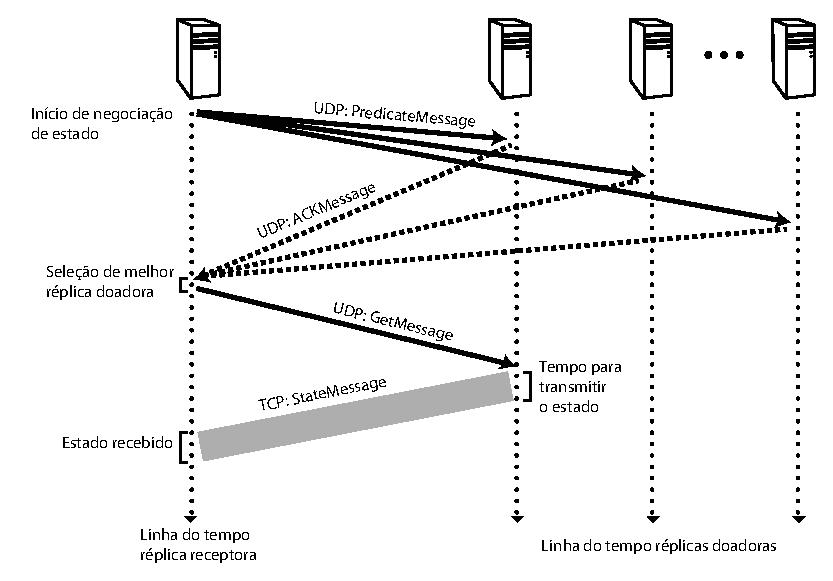
\includegraphics[width=11cm]{conteudo/capitulos/figuras/transferencia_estado.eps}
  \caption{Protocolo de transferência de estado}
  \label{fig:protocolo}
\end{figure}

\subsubsubsection{PolicyMessage}

A classe \classname{PolicyMessage} é a primeira mensagem do protocolo para transferência
de estado. Essa classe além de sinalizar para as outras réplicas do grupo que existe uma
réplica interessada em receber um estado, contém todas as informações sobre o estado
pretendido pela réplica receptora.

Os dados contratuais são abstraídos pela classe \classname{Policy}. Essa classe por sua
vez, contém o número da instância de consenso desejado (informação mínima para proposta de
um acordo) e uma lista de regras qualificadoras, que uma réplica deve atender para ser uma
doadora. O número da instância de consenso serve como identificador único de um estado por
representar a sequência de operações que foram efetivamente aplicadas, ou seja, mudaram o
estado.

\subsubsubsection{DealMessage}

Essa classe abstrai uma proposta de acordo. Ela é uma sinalização para a réplica receptora
da existência de uma réplica disposta a doar seu estado, ou seja, a réplica doadora está
em conformidade com a política estabelecida pela réplica receptora. Quanto menos
restritivas são as políticas que definem a seleção de um estado mais mensagens de acordo
serão enviadas para a réplica receptora, potencializando a seleção de uma doadora.

\subsubsubsection{GetMessage}

A classe \classname{GetMessage} é a abstração da mensagem de pedido de estado enviada
somente para a réplica doadora. As informações do endereço para envio do estado (através
de \emph{socket} TCP) são extraídas dessa mensagem.

\subsubsubsection{StateMessage}

A classe \classname{StateMessage} é a abstração do estado enviado da réplica doadora para
a réplica receptora. Essa classe possuí como atributos o número da instância de consenso,
indicando a última operação que causou alteração no estado e um estado que implementa
\classname{Serializable}. Definimos essa classe como uma cópia instantânea, tirada durante
o período que a réplica estava bloqueada para alterações.

A partir do conteúdo armazenado por \classname{StateMessage}, qualquer réplica que possuí
um estado identificado por um número de instância menor\footnote{Podemos supor comparações
de estados através da última instância de consenso, já que o mesmo é um limiar crescente
\cite{vieira-tr10b}.} pode se beneficiar da substituição de seu estado local corrente
(desatualizado) por um mais atual. Em outras palavras, a réplica receptora executa uma
operação de \emph{avanço de estado} para o estado $i$.

O avanço de estado implica na execução instantânea de uma série de operações que, do ponto
de vista da aplicação, não causam problemas de acordo com as regras de Treplica. Do ponto
de vista de Paxos, o resultado das instâncias menores que $i$ ficam potencialmente
indefinidas, mas a réplica receptora não procura ativamente decidi-las. Apenas participa
delas se for requisitada, de forma a sempre garantir o quórum.

\subsubsubsection{Diplomat}

A classe \classname{Diplomat} é responsável por implementar o tratamento das mensagens do
protocolo de trasferência. Toda réplica possui uma instância da classe
\classname{Diplomat} para representar seus interesses frente outras réplicas. A abstração
desse componente foi inspirada nas funções de diplomacia (ciência e arte referentes às
relações entre Estados \cite{aurelio}) exercidas por um Diplomata no modelo atual de
relação entre nações\footnote{Segundo \citeonline{aurelio}, diplomata é um funcionário que
representa um governo junto de outro governo.}.

O Diplomata adéqua suas funções de trabalho conforme o estado corrente da réplica. Em uma
réplica receptora, estão habilitados as funções responsáveis por obter um novo estado:
criação de política, seleção de réplica doadora e abertura de \emph{socket} TCP. Por outro
lado, em uma réplica doadora as funções para ceder o estado é que estão habilitadas:
análise de aderência a política de transferência, bloqueio de alterações de estado e o
envio de estado.

Para seleção da melhor proposta de transferência de estado o Diplomata armazena em
memória todas as propostas recebidas e após um tempo pré-estabelecido a seleção é
realizada. Consideramos como melhor proposta de estado aquela que possui maior
instância de consenso. Em caso de eventuais erros e/ou \emph{timeouts} as propostas são
removidas da memória para evitar conflitos com as futuras propostas de acordo, que serão
recebidas devido atuação do mecanismo de reinicialização.

\subsubsection{Política de Reconfiguração}

Identificamos dois potenciais pontos que se beneficiariam da utilização do protocolo de
transferência de estado: (1) expansão do aglomerado e (2) recuperação de erros. Para a
construção desse trabalho, focamos na aplicação do protocolo na expansão do aglomerado,
conforme ilustra a \autoref{fig:inclusao}. Supomos alguns aspectos para serem
considerados:

\begin{itemize}
  \item O estado da nova réplica que deseje se juntar ao aglomerado está defasado com
    relação ao estado das réplicas que já participam do grupo. É imprescindível que essa
    defasagem seja suprimida.
  \item A operação para igualar o estado da nova réplica com o estado compartilhado pelo
    grupo deve ser consistente.
  \item O impacto gerado para o processamento do aglomerado deve ser mínimo.
\end{itemize}

Para justificar a inclusão de uma nova réplica, obrigatoriamente é preciso geração de
benefícios para o processamento em grupo, caso contrário estamos executando operações sem
serventia com potencial para saturar o sistema.

\begin{figure}[ht]
  \centering
  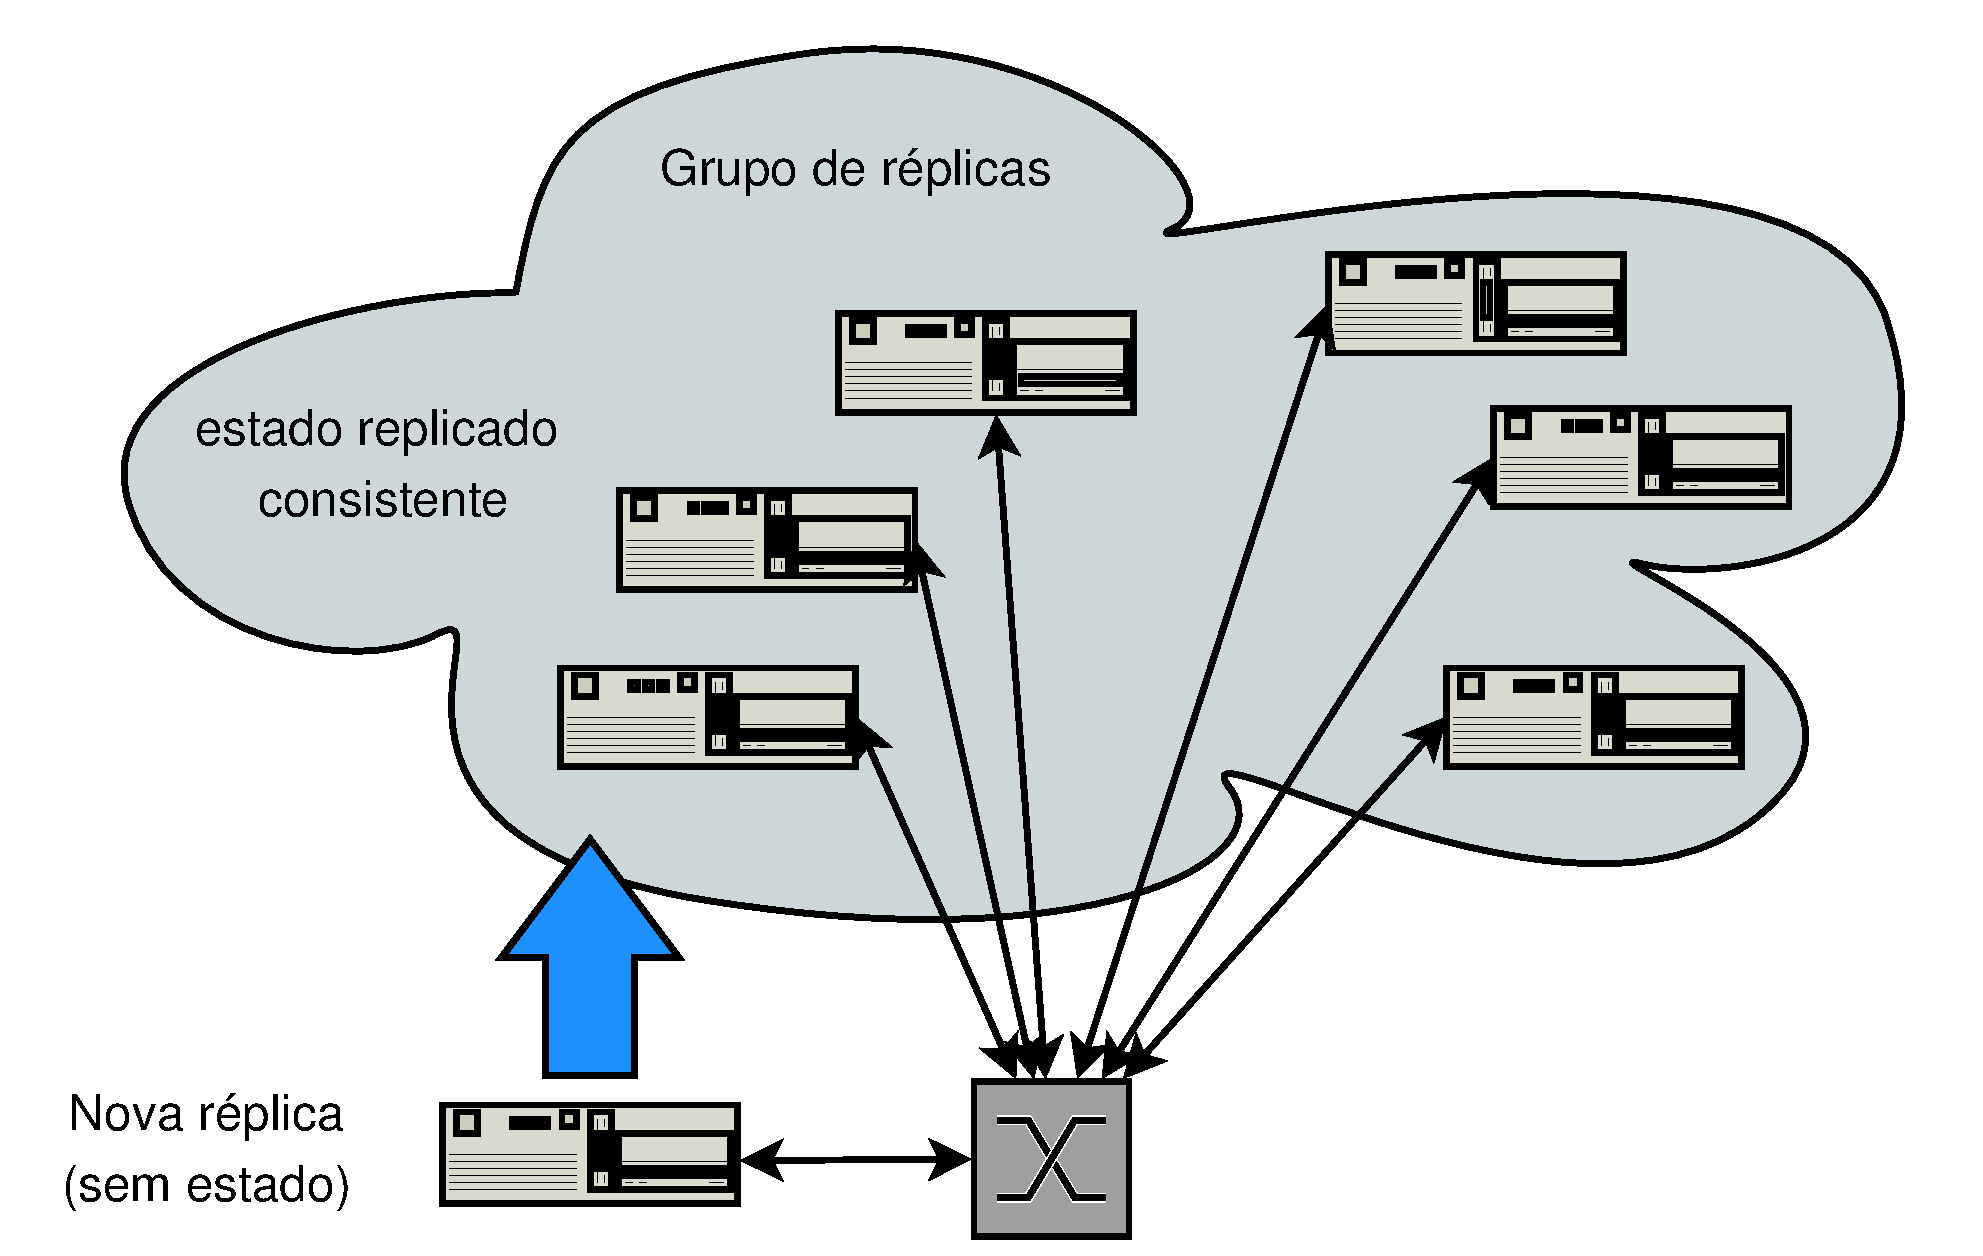
\includegraphics[width=11cm]{conteudo/capitulos/figuras/inclusao_replica_cluster.eps}
  \caption{Inclusão de réplica}
  \label{fig:inclusao}
\end{figure}

\citeonline{lamport10} apresentam um mecanismo para reconfiguração que funciona através da
criação de diferentes formações de grupos representados por visões, controladas por um
identificador sequencial. Como estamos trabalhando no modelo computacional assíncrono com
falha-e-recuperação, a aplicação dessa proposta é complexa. Se analisarmos um instante no
tempo, diferentes visões poderão estar sendo executadas simultaneamente com a visão
corrente (visão com maior identificador). O gerenciamento dessas visões e a formação de
diferentes grupos não é uma tarefa trivial.

Investimos nosso esforço na construção de um mecanismo que tenta fugir da complexidade do
mecanismo de visões proposto por \citeonline{lamport10}, consequentemente evitamos
reconfigurações em réplicas completas e focamos na criação e remoção de réplicas parciais,
que chamamos de réplicas leitoras e que serão descritas na \autoref{sec:replicas_leitoras}.

A partir da suposição de um mecanismo geral para "preenchimento de lucanas" no estado
utilizando o protocolo de transferência, as réplicas leitoras são um caso particular que
pode ser atendido por tal mecanismo, de forma que elas apenas usam transferência de estado
caso a lacuna no seu estado seja muito grande. O custo da política de reconfiguração pode
ser derivado do custo da aplicação do protocolo de transferência que está diretamente
ligado ao tamanho da lacuna que se deseja preencher.

O trabalho de especificação de parâmetros para essa política ainda está em seu estágio
inicial, dependendo de estudos mais aprofundados para caracterizar os custos envolvidos.
Outro potencial trabalho que demanda mais estudos é a criação um mecanismo capaz de
detectar lacunas no estado e selecionar a melhor forma de preenchimento de acordo com o
tamanho do buraco. Tal mecanismo poderia optar entre: (1) acionar a transferência de
estado ou (2) utilizar o mecanismo sequencial de Treplica.

\subsection{Paxos com Réplicas Leitoras}\label{sec:replicas_leitoras}

A ideia principal da abordagem proposta é utilizar o protocolo de transferência de estado
para instanciar réplicas que não participem do processo de decisão de instâncias de
consenso. A motivação por trás da criação de \emph{réplicas leitoras} é permitir que o
sistema reaja de forma autônoma a picos de carga sem comprometer o desempenho do mesmo. No
entanto, sem uma política cuidadosa de reconfiguração corre-se o risco de gastar muitos
dos recursos do sistema no próprio processo de reconfiguração, anulando quaisquer ganhos
advindos do acréscimo de novas réplicas leitoras.

A adoção de réplicas leitoras é uma subclasse do problema de reconfiguração de Paxos, no
entanto é uma forma mais simples de ser implementada pois não altera o número estático de
réplicas com o poder de alterar o estado. Definimos réplicas leitoras como réplicas onde
apenas parte dos agentes do algoritmo Paxos estão executando. Para maior clareza de
exposição, quando necessário, chamaremos as réplicas contendo todos os agentes ativos de
\emph{réplicas votantes}

\subsubsection{Réplicas Leitoras}

Réplicas leitoras são réplicas onde apenas os agentes proponente e aprendiz estão
executando. Dessa forma, do ponto de vista do conjunto de processos que implementam o
algoritmo Paxos, uma réplica leitora é capaz apenas de propor operações a serem aplicadas
no estado replicado e de aprender operações decididas pelo conjunto de receptores. Do
ponto de vista do cliente da aplicação replicada um réplica leitora se comporta como uma
réplica votante: ela atende requisições de qualquer tipo garantindo a execução atômica das
mesmas.

As réplicas leitoras não assumem um papel fundamental na execução do algoritmo Paxos, no
entanto elas se integram de forma consistente com a operação das réplicas votantes por
meio de suas funções fundamentais: propor e aprender requisições de escrita. As réplicas
leitoras propõem novas requisições a serem executadas em nome de seus clientes através de
seu agente proponente. O proponente encaminha a operação ao coordenador que por sua vez
decide, em conjunto com os receptores, a ordem da mesma através de uma rodada de Paxos,
como descrito na \autoref{sec:paxos}. Uma vez que a decisão é alcançada, a mesma é
difundida para o resto do sistema. Nesse momento o agente aprendiz da réplica leitora toma
conhecimento da decisão e atualiza o seu estado interno, sem a participação ativa do
coordenador ou de qualquer receptor.

Tanto o processo de proposta quanto o de aprendizado executado por uma réplica leitora
devem usar as mesmas estratégias de implementação das réplicas votantes. Na verdade, em
nossa implementação usando Treplica, as réplicas leitoras foram construídas a partir da
separação modular dos agentes que implementam Paxos. Dessa forma, reutilizamos os mesmos
componentes e por consequência essas réplicas são capazes de detectar e reenviar propostas
perdidas, detectar e corrigir lacunas na sequência de instâncias de consenso, fazer
controle de fluxo e de congestionamento, entre outras operações fundamentais para uma
operação eficiente de Paxos \cite{vieira-tr10b}.

Uma consequência importante do uso de réplicas leitoras é que essas réplicas,
consistentemente com as funções que elas assumem no algoritmo Paxos, não precisam de
memória persistente para sua operação. Isso se deve ao fato de que elas não executam as
Fases 1 e 2 do algoritmo, descrito na \autoref{sec:paxos}. Porém, pode ser interessante
que essas réplicas registrem a proposta decidida de forma a não precisar realizar uma
recuperação completa em caso de falha. Na nossa proposta de réplicas leitoras decidimos
não fazer esse registro de forma a remover completamente a escrita em memória persistente
do caminho crítico de execução. É interessante observar que a escrita eliminada ocorre
somente quando a réplica leitora atualiza o seu estado de acordo com as propostas
decididas pelos receptores das réplicas votantes. Dessa forma, as réplicas leitoras
conseguem manter seu estado atualizado com as réplicas votantes com um custo mínimo. Elas
também são capazes de processar requisições de escrita com um custo similar àquele gerado
pelas réplicas votantes ao executar as mesmas requisições. Podemos argumentar que esse
custo é menor, na medida que as réplicas leitoras aliviam as réplicas votantes do custo de
manter as conexões abertas com os clientes.

Utilizando réplicas leitoras, podemos formar grupos de réplicas com diferentes graus de
uso de memória persistente \cite{aguilera00}. Uma configuração simples seria mesclar
réplicas votantes e leitoras formando um conjunto híbrido de réplicas transparente para o
cliente, conforme ilustra a \autoref{fig:configuracao_replicas_leitoras} (a). É concebível
ainda uma configuração onde as réplicas votantes não entram em contato com os clientes,
sendo essa operação completamente delegada às replicas leitoras, configuração ilustrada
pela \autoref{fig:configuracao_replicas_leitoras} (b).

\begin{figure}[ht]
  \begin{center}
    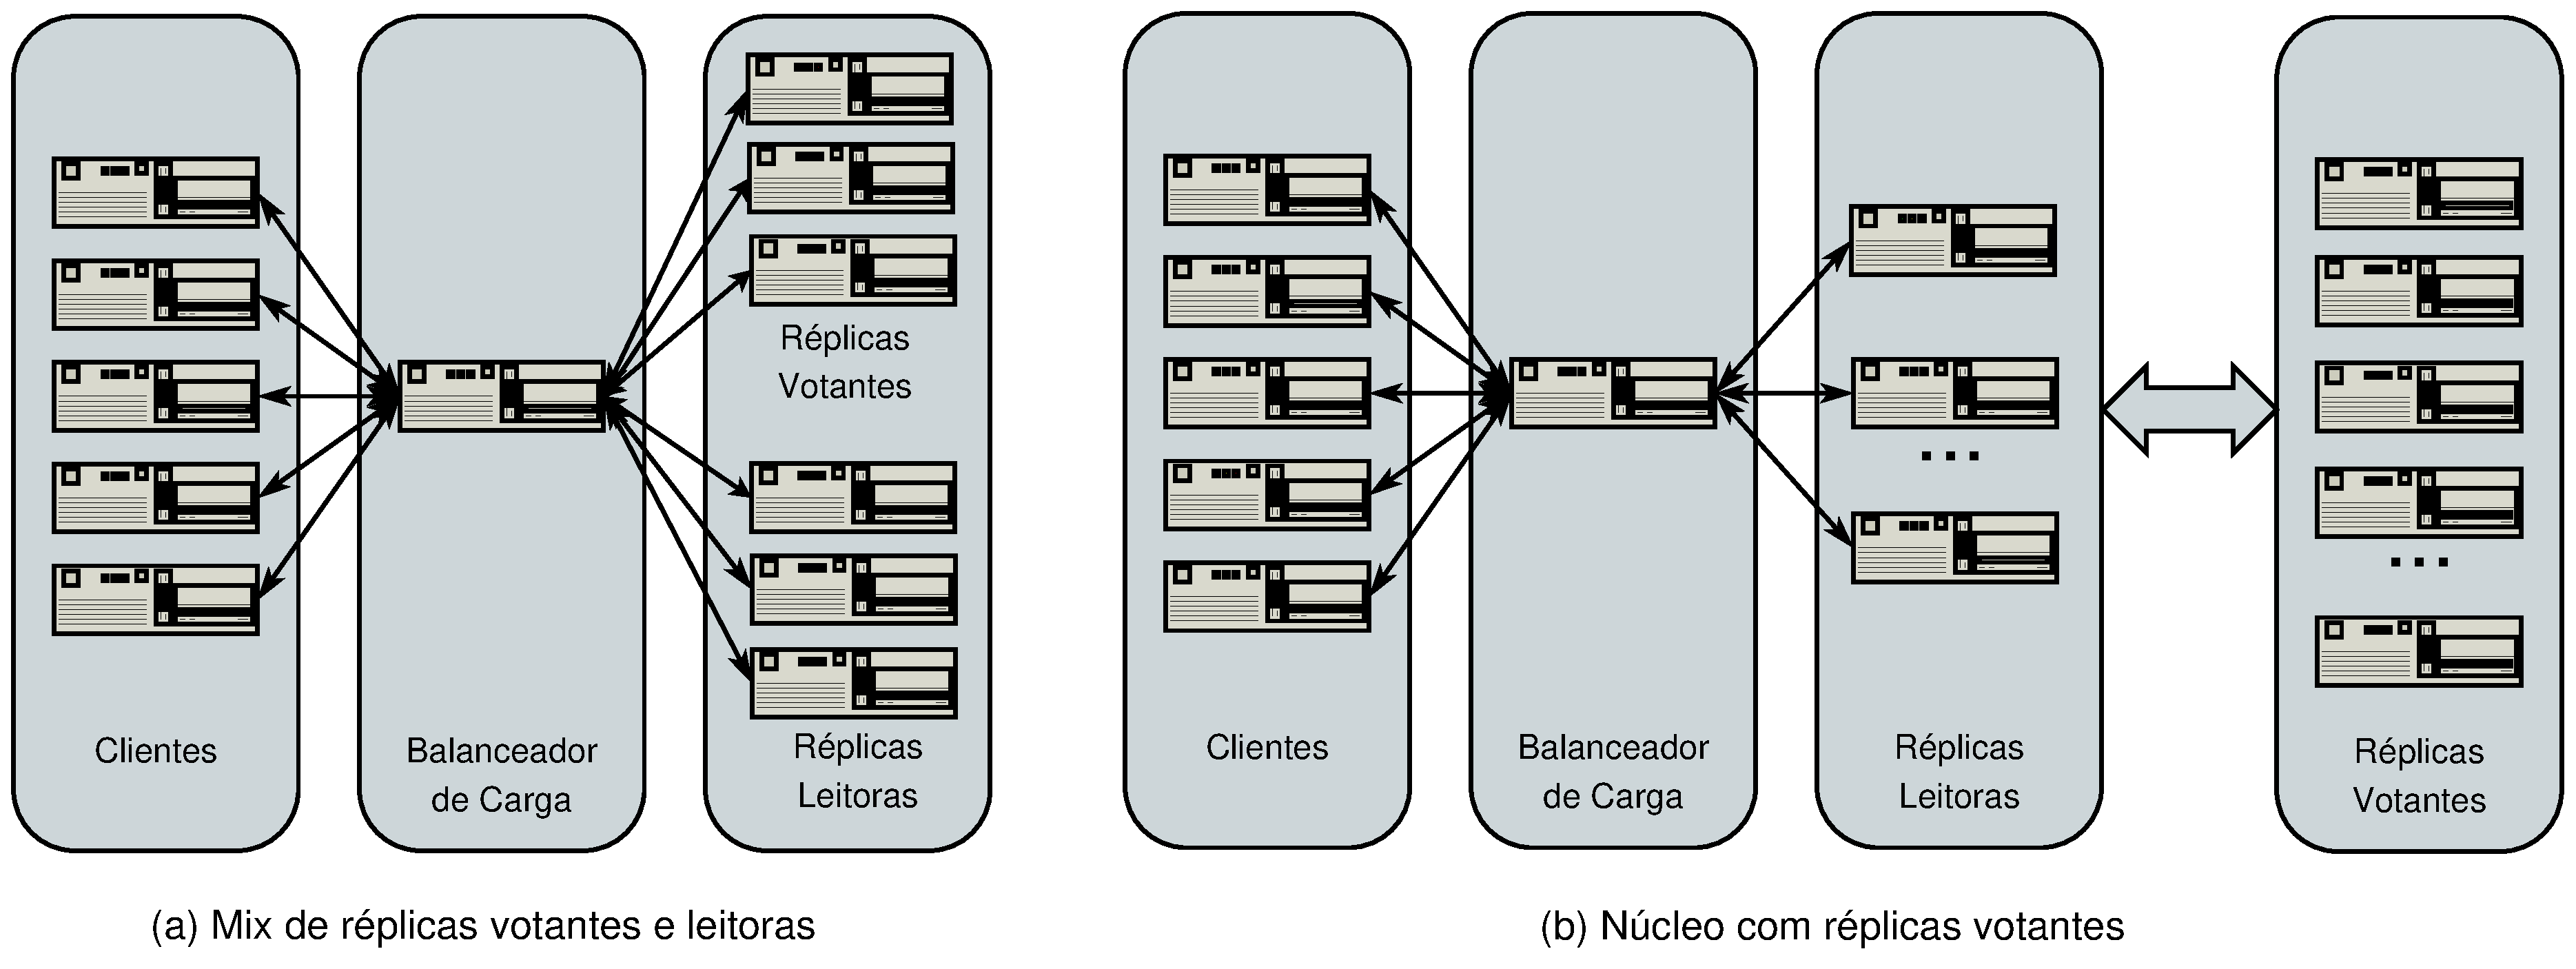
\includegraphics[width=16cm]{conteudo/capitulos/figuras/configuracao_replicas_leitoras.eps}
  \end{center}
  \caption{Configuração de Paxos com réplicas votantes e leitoras}
  \label{fig:configuracao_replicas_leitoras}
\end{figure}

As réplicas leitoras funcionam então como uma espécie de cache \emph{write-through}
distribuído. O estado replicado na memória destas réplicas permite atender diretamente as
requisições de leitura dos clientes, enquanto as requisições de escrita são repassadas ao
receptores. Podemos ver claramente que a taxa de acerto desse cache está diretamente
ligada à proporção de operações de leitura geradas pelos clientes e que a vazão de
operações de leitura tem o potencial de crescer linearmente com o número de réplicas
leitoras disponíveis.

\subsubsection{Implementação}

Originalmente, uma única configuração de réplicas que empregava todos os agentes de Paxos
utilizando memória persistente, conforme descrito na \autoref{subsec:agentes_paxos}. Para
implementar réplicas leitoras foi necessário alterar a forma como é feita o agrupamento de
agentes.

A classe denominada \classname{PaxosPersistentQueue} é responsável por implementar o
agrupamento de todos os agentes de Paxos, caracterizando assim uma réplica votante. Uma
réplica votante possui como uma das suas \emph{threads} ativas o \emph{main loop} da classe
\classname{PaxosPersistentQueue}, como descrito na \autoref{subsec:agentes_paxos}. Em
contra partida, uma réplica leitora executa o \emph{main loop} da classe
\classname{PaxosReadonlyQueue}. Essa classe, implementa somente a agregação dos agentes
proponente e aprendiz, sem a utilização de memória persistente. Detalharemos nas próximas
seções a implementação proposta para esse componente.

\subsubsubsection{PaxosReadonlyQueue}

A classe \classname{PaxosReadonlyQueue} foi criada para fornecer o mesmo comportamento da
classe \classname{PaxosPersistenteQueue}: disponibilizar uma fila assíncrona usando o
algoritmo Paxos. Dessa forma, as operações suportadas por \classname{PaxosReadonlyQueue}
são as mesmas. Do ponto de vista do processamento de mensagens postadas na fila, as
seguintes propriedades caracterizam uma réplica leitora:

\begin{itemize}
  \item Abdicar liderança: todas as mensagens relacionadas a eleição de líder não são
    processadas, logo é eliminada qualquer possibilidade de uma réplica leitora se tornar
    coordenadora de uma rodada de Paxos.
  \item Inelegível ao voto: mensagens relacionadas a votação de uma proposta são
    ignoradas. Dessa forma, réplicas leitoras não participam do processo de decisão de
    consenso e não são essenciais para o progresso do algoritmo Paxos.
  \item Aprendizado: todas as mensagens endereçadas ao componente \classname{Learner} são
    processadas pela fila. Consequentemente, os mecanismos para descobrir qual foi o
    consenso de uma determinada rodada são habilitados.
\end{itemize}

O principal objetivo dessa classe é participar das operações que não exigem dados
persistentes para garantir correção do algoritmo, oferecendo instâncias capazes de atuar
parcialmente nas fases de Paxos. Do ponto de vista do cliente da aplicação um réplica
leitora se comporta como uma réplica votante: ela atende requisições de qualquer tipo
garantindo a execução atômica das mesmas. Sendo assim, as seguintes premissas não podem
ser violadas:

\begin{itemize}
  \item Mensagens quem alteram o estado (escrita): são resolvidas pelo aglomerado de
    réplicas orquestrado pelo protocolo Paxos.
  \item Mensagens que não alteram estado (leitura): são resolvidas localmente independente
    do grau de memória da réplica.
\end{itemize}

Do ponto de vista de uma réplica votante, não é possível distinguir se a proposta é
oriunda de uma réplica votante ou leitora. Como Treplica utiliza mecanismo de difusão para
enviar as mensagens de Paxos, uma nova réplica conectada na rede passa a receber todas as
mensagens do protocolo. A réplica leitora está programada para ignorar as mensagens de
formação de quórum e processar somente as mensagens roteadas para seus agentes ativos:
proponente e aprendiz. Dessa forma, garantimos que as instâncias de consenso são lidas por
todas as máquinas, garantindo a transparência da adoção de réplicas leitoras e podemos
afirmar que o progresso e a correção de Paxos não são violados.

A principal razão para a criação dessa abstração em Treplica foi eliminar a operação de
persistência em disco, gerando um componente volátil, capaz de oferecer as operações
essenciais para o progresso do algoritmo sem o ônus da escrita em disco.

\subsubsubsection{WeakSecretary}

A classe \classname{WeakSecretary} apresenta uma abstração de I/O sem persistência de
dados em disco. Esse componente é uma versão leve da classe \classname{Secretary}, que é
utilizada pelos agentes de Paxos para enviar mensagens pela rede, através do intermédio do
componente \classname{Transport}. Essa classe foi projetada para trabalhar com dados
somente em memória, dessa forma todos os dados normalmente encaminhados a memória
persistente são perdidos na presença de defeitos na réplica. No entanto, na ausência de
falhas nos beneficiamos da eliminação de uma operação custosa relacionada com E/S em
disco.

\classname{WeakSecretary} também é responsável por lidar com o componente
\classname{Ledger} e com a fila de objetos utilizada para entregar mensagens para a camada
da aplicação. Essa classe utiliza a implementação \classname{TransientLedger} para
fornecer informações sobre os decretos conhecidos. Essa implementação fornece uma
abstração capaz de trabalhar com um estado transplantado e responde \classname{null} para
todas as solicitações que utilizam um número de decreto menor que o decreto ligado ao
estado transplantado. Em outras palavras, do ponto de vista de uma réplica leitora, é
tolerável não saber o que aconteceu em instâncias de consenso anteriores ao seu estado
inicial.

O comportamento mais importante dessa classe é que eliminamos a fila de escalonamento de
entrada e saída, sendo todas as operações concluídas de modo síncrono.

\subsubsection{Provisionamento de Réplicas Leitoras}

É possível utilizar os mecanismos tradicionais de Treplica para provisionar uma nova
réplica leitora. Em resumo, uma réplica que se integra ao sistema pela primeira vez ou
após uma falha demorada deve recuperar o seu estado. Esse processo acontece através de um
mecanismo de preenchimento de lacunas, que observa que não pode executar novas requisições
de escrita sem antes executar as requisições anteriores \cite{vieira-tr10b}.

Esse procedimento de recuperação é voltado para reparar pequenas interrupções e não a
recuperação do estado completo de uma réplica. Em particular, no caso de uma réplica
leitora sem estado persistente, o tamanho dessa recuperação pode ser muito grande em
termos do número de \emph{requisições} a serem reexecutadas, pois ela sempre parte do
estado inicial vazio.

Decidimos então usar sempre o protocolo de transferência de estado para provisionar uma
réplica leitora, pois com apenas esse mecanismo podemos configurar réplicas independente
da sua classificação: votante ou leitora. Porém nessa versão, o mecanismo de transferência
de estado é aplicado somente para réplicas leitoras. A configuração desse tipo de réplica
se torna mais fácil pelo fato de uma réplica não ter estado persiste (nada precisa ser
recuperado do disco). Em particular, a adição ou remoção de uma réplica leitora não altera
o número de receptores executando o algoritmo, não havendo necessidade de se realizar um
reconfiguração custosa \cite{lamport10}.

\subsection{Transferência de estado para recuperação de falhas}

Treplica possui outro potencial candidato para empregar o protocolo de transferência de
estado: o componente detector de lacunas na sequência de instâncias de consenso. Lacunas
podem surgir por diferentes motivos: falha-e-recuperação na réplica, perda de mensagens ou
ainda réplicas com grandes diferenças de capacidade de processamento. Para preencher
lacunas detectadas o componente solicita retransmissão da instância de consenso em uma
determinada rodada. É perceptível que na presença de grandes lacunas essa abordagem
exigirá uma longa sequência de retransmissões.

Para exemplificar o potencial problema do detector de lacunas, vamos supor que uma
aplicação está passando por um grande pico de processamento (\emph{flash crowds}) e que a
réplica $r$ possui uma grande lacuna. O mecanismo detector de lacunas solicitará
retransmissão das instâncias de consenso não conhecidas por $r$, aumentando a concorrência
no meio compartilhado pelas réplicas: a rede. Como solução alternativa, podemos utilizar o
mecanismo de transferência para concentrar em uma única mensagem o estado resultante da
execução das operações codificadas pelas instâncias de consenso. Dessa forma, um mecanismo
de detecção de lacunas deveria ter a capacidade de:

\begin{itemize}
  \item Retransmissão de instância de consenso: utilizado para preencher pequenas lacunas
    na sequência de consenso.
  \item Protocolo de transferência de estado: utilizado para preencher grandes lacunas,
    onde retransmissão tem potencial perda de desempenho.
\end{itemize}

